\documentclass[11pt,oneside]{article}
\usepackage[margin=1in]{geometry}
\usepackage{booktabs}
\usepackage{graphicx}
\usepackage{amsmath}
\usepackage{array}
\usepackage{caption}
\usepackage{float}
\usepackage[T1]{fontenc}
\usepackage{newtxtext,newtxmath}
\usepackage{microtype}
\usepackage{setspace}
\setstretch{1.08}
\setlength{\parindent}{1.5em}
\setlength{\parskip}{0.25em}
\captionsetup{font=small,labelfont=bf}
\graphicspath{{./}}

\title{\textbf{Machine-Learning Prediction of Young's Modulus of Titanium Alloys from Chemical Composition}}
\author{\texttt{<TODO: author name>}\\
\texttt{<TODO: department, college>}\\[0.5em]
Supervisor: \texttt{<TODO: professor name>}}
\date{\texttt{<TODO: date>}}

\begin{document}
\maketitle

\begin{abstract}
Low Young's modulus in beta-titanium alloys is desirable for biomedical implants because it can reduce stress shielding. Experimental modulus measurement is slow, while composition--property measurements are scattered across sources. This study evaluated whether chemical composition in weight percent, with a small set of derived descriptors, could predict Young's modulus, \(E\), in GPa. Fifteen CSV files were merged into an experimental table. Computed rows were excluded, rows were filtered by atomic titanium content, and repeated compositions were collapsed by their median modulus before a grouped train/test split. A composition-plus-engineered-feature XGBoost regressor with an absolute-error objective and default parameters was selected using five-fold grouped cross-validation on the training data. On the held-out test set of 151 rows, it obtained an MAE of 9.88 GPa, an RMSE of 13.00 GPa, and an \(R^2\) of 0.684. The test MAE was approximately 1.12 times the estimated 8.78 GPa within-composition noise floor. Engineered features did not clearly improve grouped-CV error over composition alone. The results support composition-based screening, but not processing-independent material-property claims.
\end{abstract}

\section{Introduction}
Titanium alloys are used in biomedical implants, where a lower elastic modulus can reduce the stiffness mismatch with bone and thereby reduce stress shielding. Beta-titanium alloys are of particular interest in this context. Young's modulus is commonly measured experimentally, but measurement is slow and values reported in the literature are dispersed across papers and experimental methods. A composition-based predictor could help prioritize candidate compositions for further measurement; it cannot replace experiments that account for processing and phase constitution. [reference needed]

The objective was to predict \(E\) in GPa from alloy composition in weight percent. The analysis compared elemental composition alone with a composition-plus-engineered feature set. Model selection used only the training partition and composition-grouped folds; the held-out test set was used once for final evaluation. The report describes the data curation, feature definitions, validation results, and limits of interpretation.

\section{Data}
The initial merged table contained 897 rows from 15 CSV files. The sources comprised literature compilations, earlier project datasets, values digitized from published figures, and density-functional-theory (DFT) values from Materials Project and two DFT figures. Figure-digitized values had an estimated reading error of approximately \(\pm 0.5\) to \(2\) GPa. Compositions were represented in wt\% and the target was \(E\) in GPa. Any at\% compositions were converted to wt\% using standard atomic masses, and rows were normalized to 100 wt\%.

Computed values were excluded because they sat systematically apart from experimental values: 38 rows were matched to the Materials Project file and 11 to the two DFT figures, for 49 removed rows. This left 848 rows. The dataset was then restricted to Ti-matrix alloys using an atomic-titanium threshold of at least 60 at\%; 31 rows, including intermetallics such as Ti--Si, Ti--Al, and Ti--Fe, were removed. The resulting 817 rows retained heavy-element beta alloys that would have been lost under a wt\%-based titanium cutoff. For example, Ti--29Nb--13Ta--4.6Zr contained 53.4 wt\% Ti but approximately 72 at\% Ti.

Compositions equal after rounding all element wt\% values to one decimal place were grouped. One record per composition was retained, with the group's median \(E\). This reduced 817 rows to 754 composition groups. Thirty groups contained more than one modulus value; their mean within-group sample standard deviation was 8.78 GPa. This quantity was treated as an empirical label-noise floor, not as a strict lower bound on achievable prediction error.

The groups were divided once using an 80/20 GroupShuffleSplit with seed 42. A rounded composition group could not occur in both partitions. The training partition contained 603 rows and the test partition 151 rows. Table~\ref{tab:split} summarizes the target distributions.

\begin{table}[H]
\centering
\caption{Target distribution in the grouped train/test split.}
\label{tab:split}
\begin{tabular}{lrrrrr}
\toprule
Partition & \(n\) & Mean (GPa) & SD (GPa) & Minimum (GPa) & Maximum (GPa)\\
\midrule
Train & 603 & 73.1 & 19.8 & 23.0 & 157.0\\
Test & 151 & 75.7 & 23.2 & 29.5 & 149.0\\
\bottomrule
\end{tabular}
\end{table}
The test partition included 46 rows with Ti below 70 wt\%. This descriptive cutoff was reported for subgroup evaluation; it was not the inclusion rule, which was based on Ti at\%.

\section{Methods}
\subsection{Composition-derived descriptors}
Feature set A contained all element wt\% columns. Feature set B contained set A and valence electron concentration (VEC), atomic-size mismatch \(\delta_r\), ideal configurational mixing entropy \(\delta S_{\mathrm{mix}}\), molybdenum equivalent (\(\mathrm{Mo}_{eq}\)), aluminium equivalent (\(\mathrm{Al}_{eq}\)), and Morinaga \(B_o\) and \(M_d\) descriptors. The set also included a coarse phase-screening label, \texttt{phase\_est}. The label used Mo-equivalent thresholds of 2.5 and 10 wt\%; it was marked uncertain when \(\mathrm{Al}_{eq}\geq 8\) wt\% or the alloy was Ti-poor (the operational threshold was not specified in the supplied report facts). The precise formulas are given in the Appendix.

For the atomic descriptors, weight compositions were converted to atomic fractions \(x_i\) using standard atomic masses after normalization. The saved inference pipeline handled the categorical \texttt{phase\_est} feature. No test-set values were used to fit feature preprocessing or select model parameters.

\subsection{Models and validation}
The evaluated model families were XGBoost regressors with squared-error and absolute-error objectives, Random Forest, Ridge, and a mean-predictor baseline. Ridge results were not included because they were not available in the v2 report. Five-fold GroupKFold cross-validation used the training partition only; groups were compositions rounded to one decimal place. Mean absolute error (MAE) was the primary selection metric; RMSE and \(R^2\) were also recorded. RandomizedSearchCV used 60 iterations for XGBoost with the absolute-error objective on feature sets A and B. The held-out test set was evaluated after model selection.

The final model was the XGBoost regressor using feature set B, objective \texttt{reg:absoluteerror}, and default parameters. The reported software versions were pandas 3.1.0, NumPy 2.5.3, scikit-learn 1.9.1, and XGBoost 3.4.1. The random seed was 42.

\section{Results}
\subsection{Cross-validation and model selection}
Table~\ref{tab:cv} reports grouped cross-validation MAE. The default feature-set B XGBoost model with the absolute-error objective had a mean MAE of 10.19 GPa (SD 0.63 GPa). Random Forest obtained 10.40 GPa (SD 0.97 GPa) with set A and 10.21 GPa (SD 1.14 GPa) with set B. The mean-predictor baseline obtained 15.39 GPa (SD 1.24 GPa) for both feature sets. The tuned absolute-error XGBoost models obtained 10.59 GPa (SD 0.77 GPa) for A and 10.43 GPa (SD 0.91 GPa) for B; tuning therefore did not improve on the selected default B model.

\begin{table}[H]
\centering
\caption{Five-fold grouped-CV MAE on the training partition. Values are mean \(\pm\) fold SD in GPa.}
\label{tab:cv}
\begin{tabular}{llr}
\toprule
Feature set & Model & MAE (GPa)\\
\midrule
A & XGBoost, absolute error & \(11.10 \pm 0.46\)\\
A & XGBoost, squared error & \(11.20 \pm 0.29\)\\
A & Random Forest & \(10.40 \pm 0.97\)\\
A & Mean baseline & \(15.39 \pm 1.24\)\\
B & XGBoost, absolute error & \(10.19 \pm 0.63\)\\
B & XGBoost, squared error & \(10.79 \pm 0.92\)\\
B & Random Forest & \(10.21 \pm 1.14\)\\
B & Mean baseline & \(15.39 \pm 1.24\)\\
A & Tuned XGBoost, absolute error & \(10.59 \pm 0.77\)\\
B & Tuned XGBoost, absolute error & \(10.43 \pm 0.91\)\\
\bottomrule
\end{tabular}
\end{table}

The selected model's test MAE was 9.88 GPa, RMSE was 13.00 GPa, and \(R^2\) was 0.684 (\(n=151\)). Its subgroup MAE was 7.78 GPa for 28 rows labelled beta by the screening rule, 11.51 GPa for 41 rows with \(E<60\) GPa, and 7.80 GPa for 46 rows with Ti below 70 wt\%.

\begin{figure}[H]
\centering
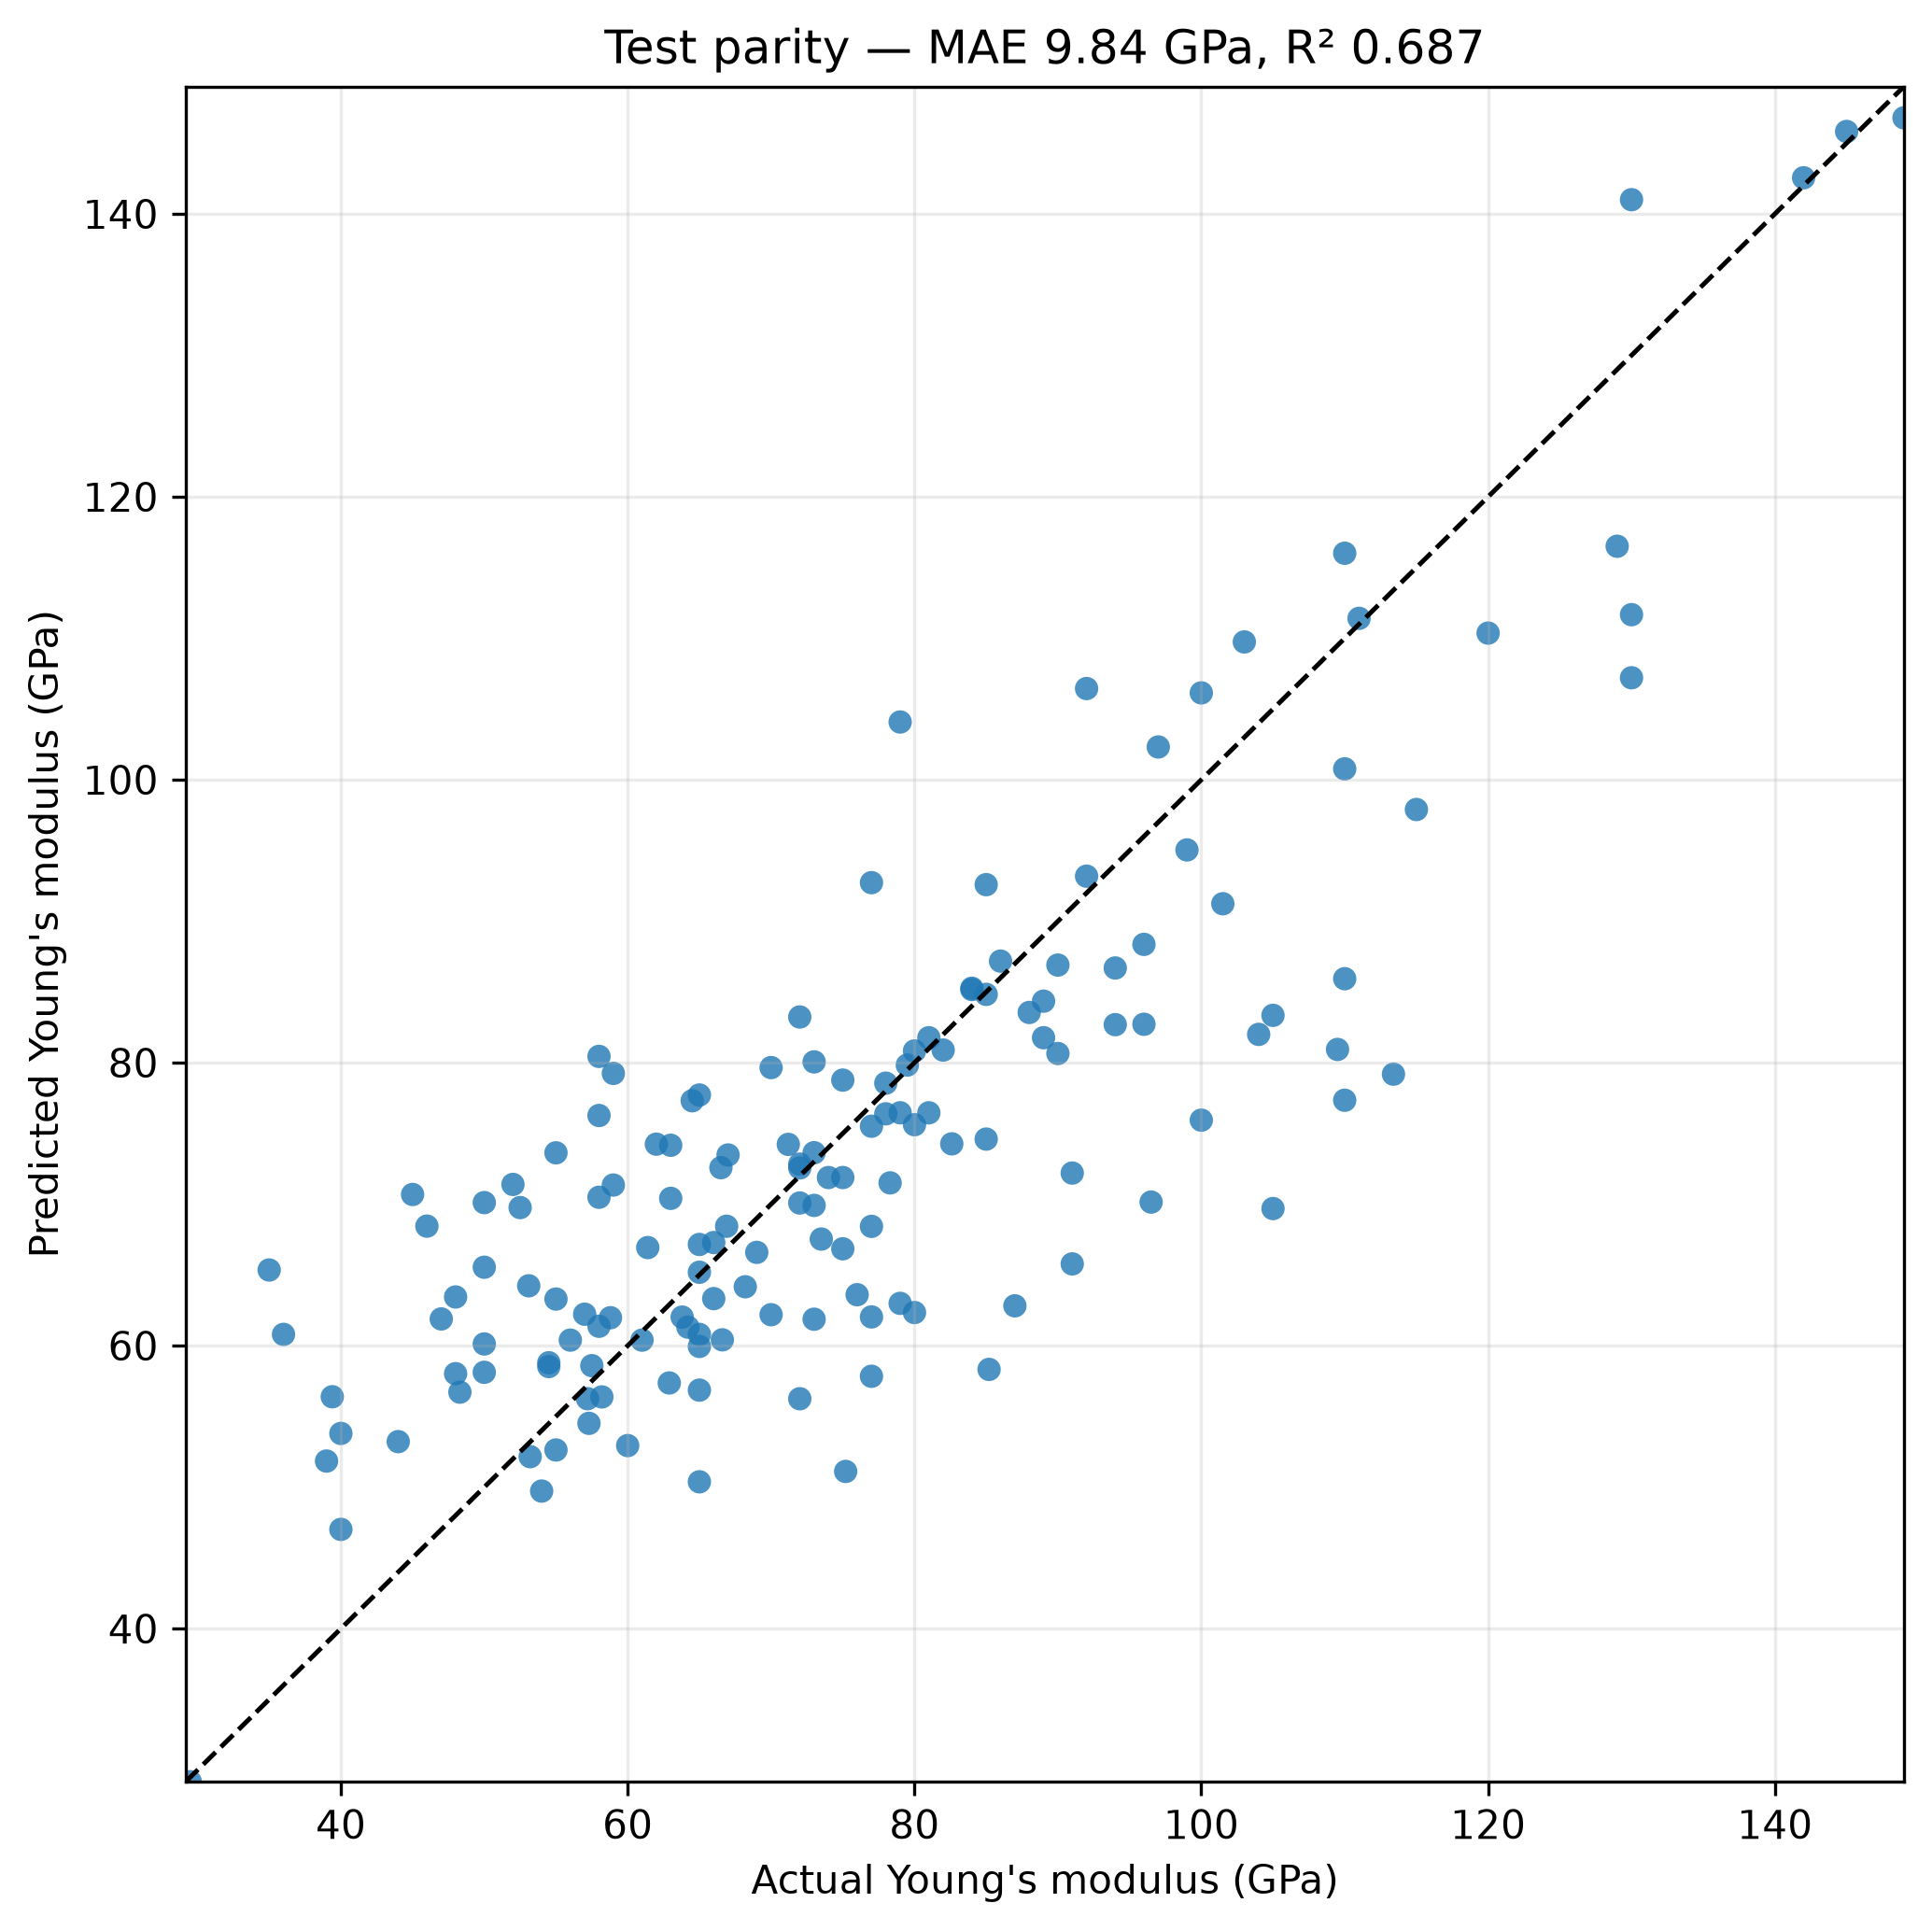
\includegraphics[width=0.70\linewidth]{parity_test.png}
\caption{Parity plot for the held-out test set. The diagonal denotes agreement between observed and predicted modulus; the title reports test MAE and \(R^2\).}
\label{fig:parity}
\end{figure}

\subsection{Composition-series plots and feature comparison}
The mean paired MAE gain from B over A was 0.17 GPa, smaller than one fold standard deviation for the tuned B model (0.91 GPa). Thus, the engineered descriptors did not clearly improve performance over composition alone.

Figure~\ref{fig:nbzr} compares model curves against digitized Ti--Nb--\(x\)Zr data for \(x=0, 4, 8, 12,\) and \(18\) at.\% Zr. The supplied point-overlap check found 28 of 44 points matching training rows within 0.5 wt\% composition and 0.5 GPa in \(E\). The plotted comparison therefore includes training observations and represents fit to a partly overlapping set, not independent validation. The file \texttt{test\_report.txt} was not present when this report was prepared; the overlap count came from the explicit comparison against \texttt{train\_v2.csv}.

\begin{figure}[H]
\centering
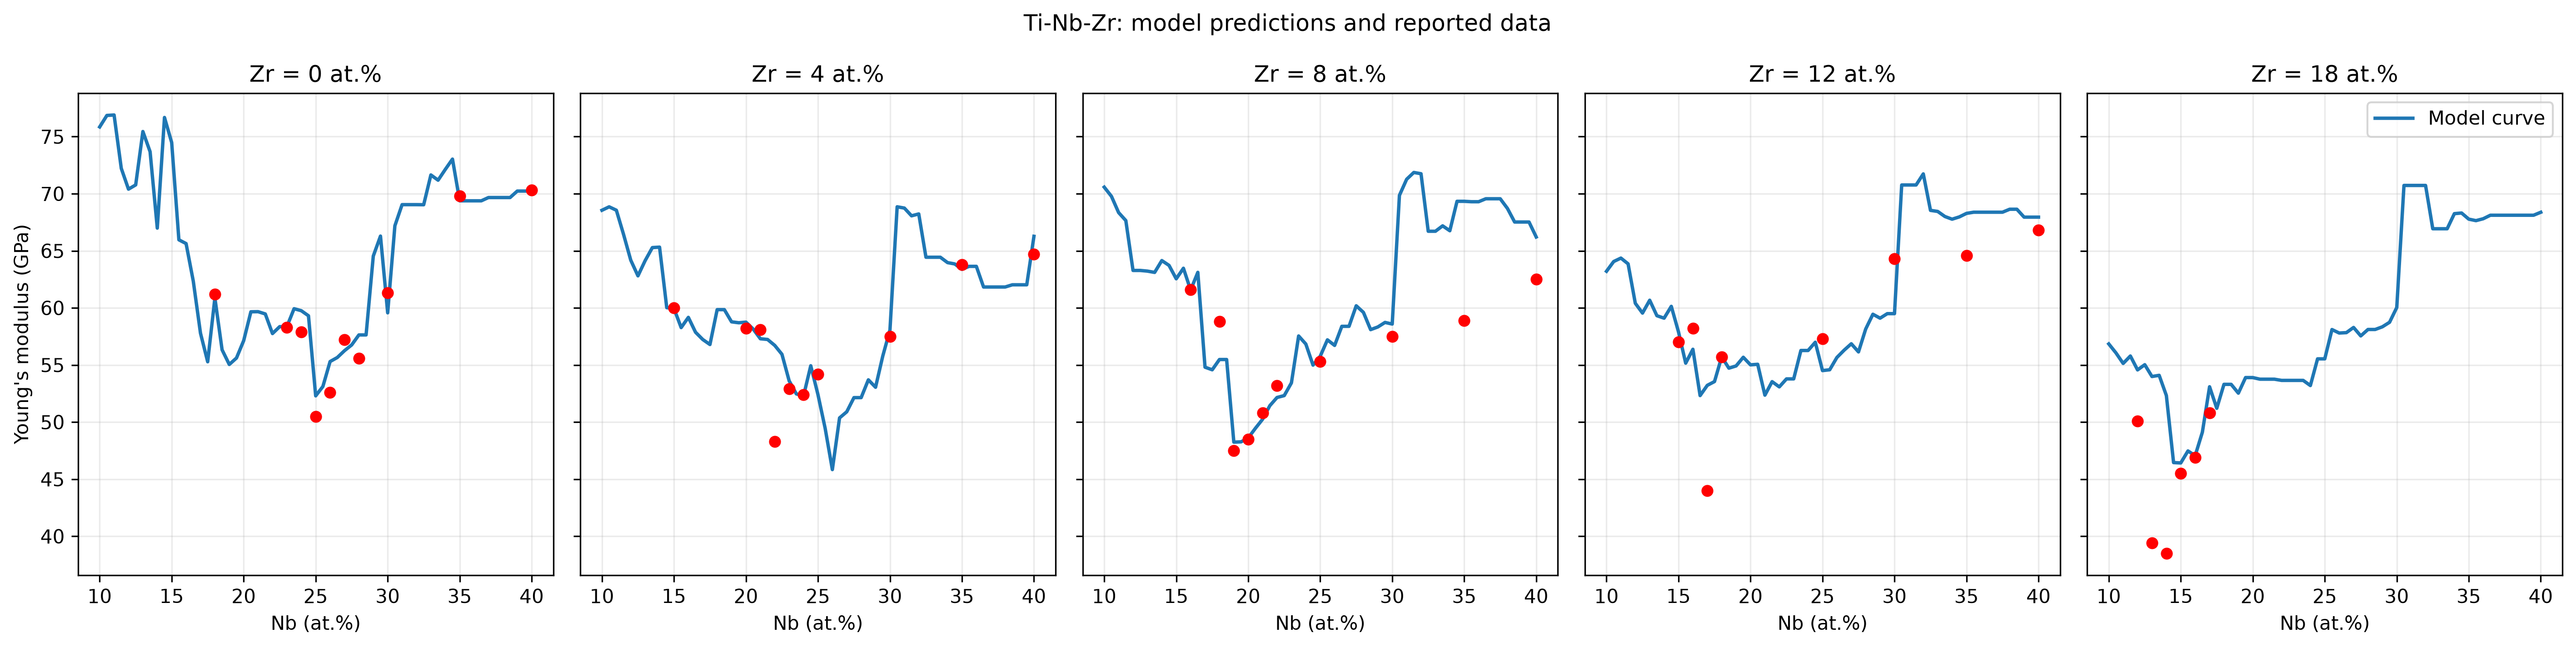
\includegraphics[width=\linewidth]{nb_zr_vs_real.png}
\caption{Predicted Ti--Nb--\(x\)Zr curves and digitized literature points at five Zr atomic-percent levels. Since 28 of 44 supplied points matched training rows at the stated tolerances, this is a partly in-sample fit visualization.}
\label{fig:nbzr}
\end{figure}

\begin{figure}[H]
\centering
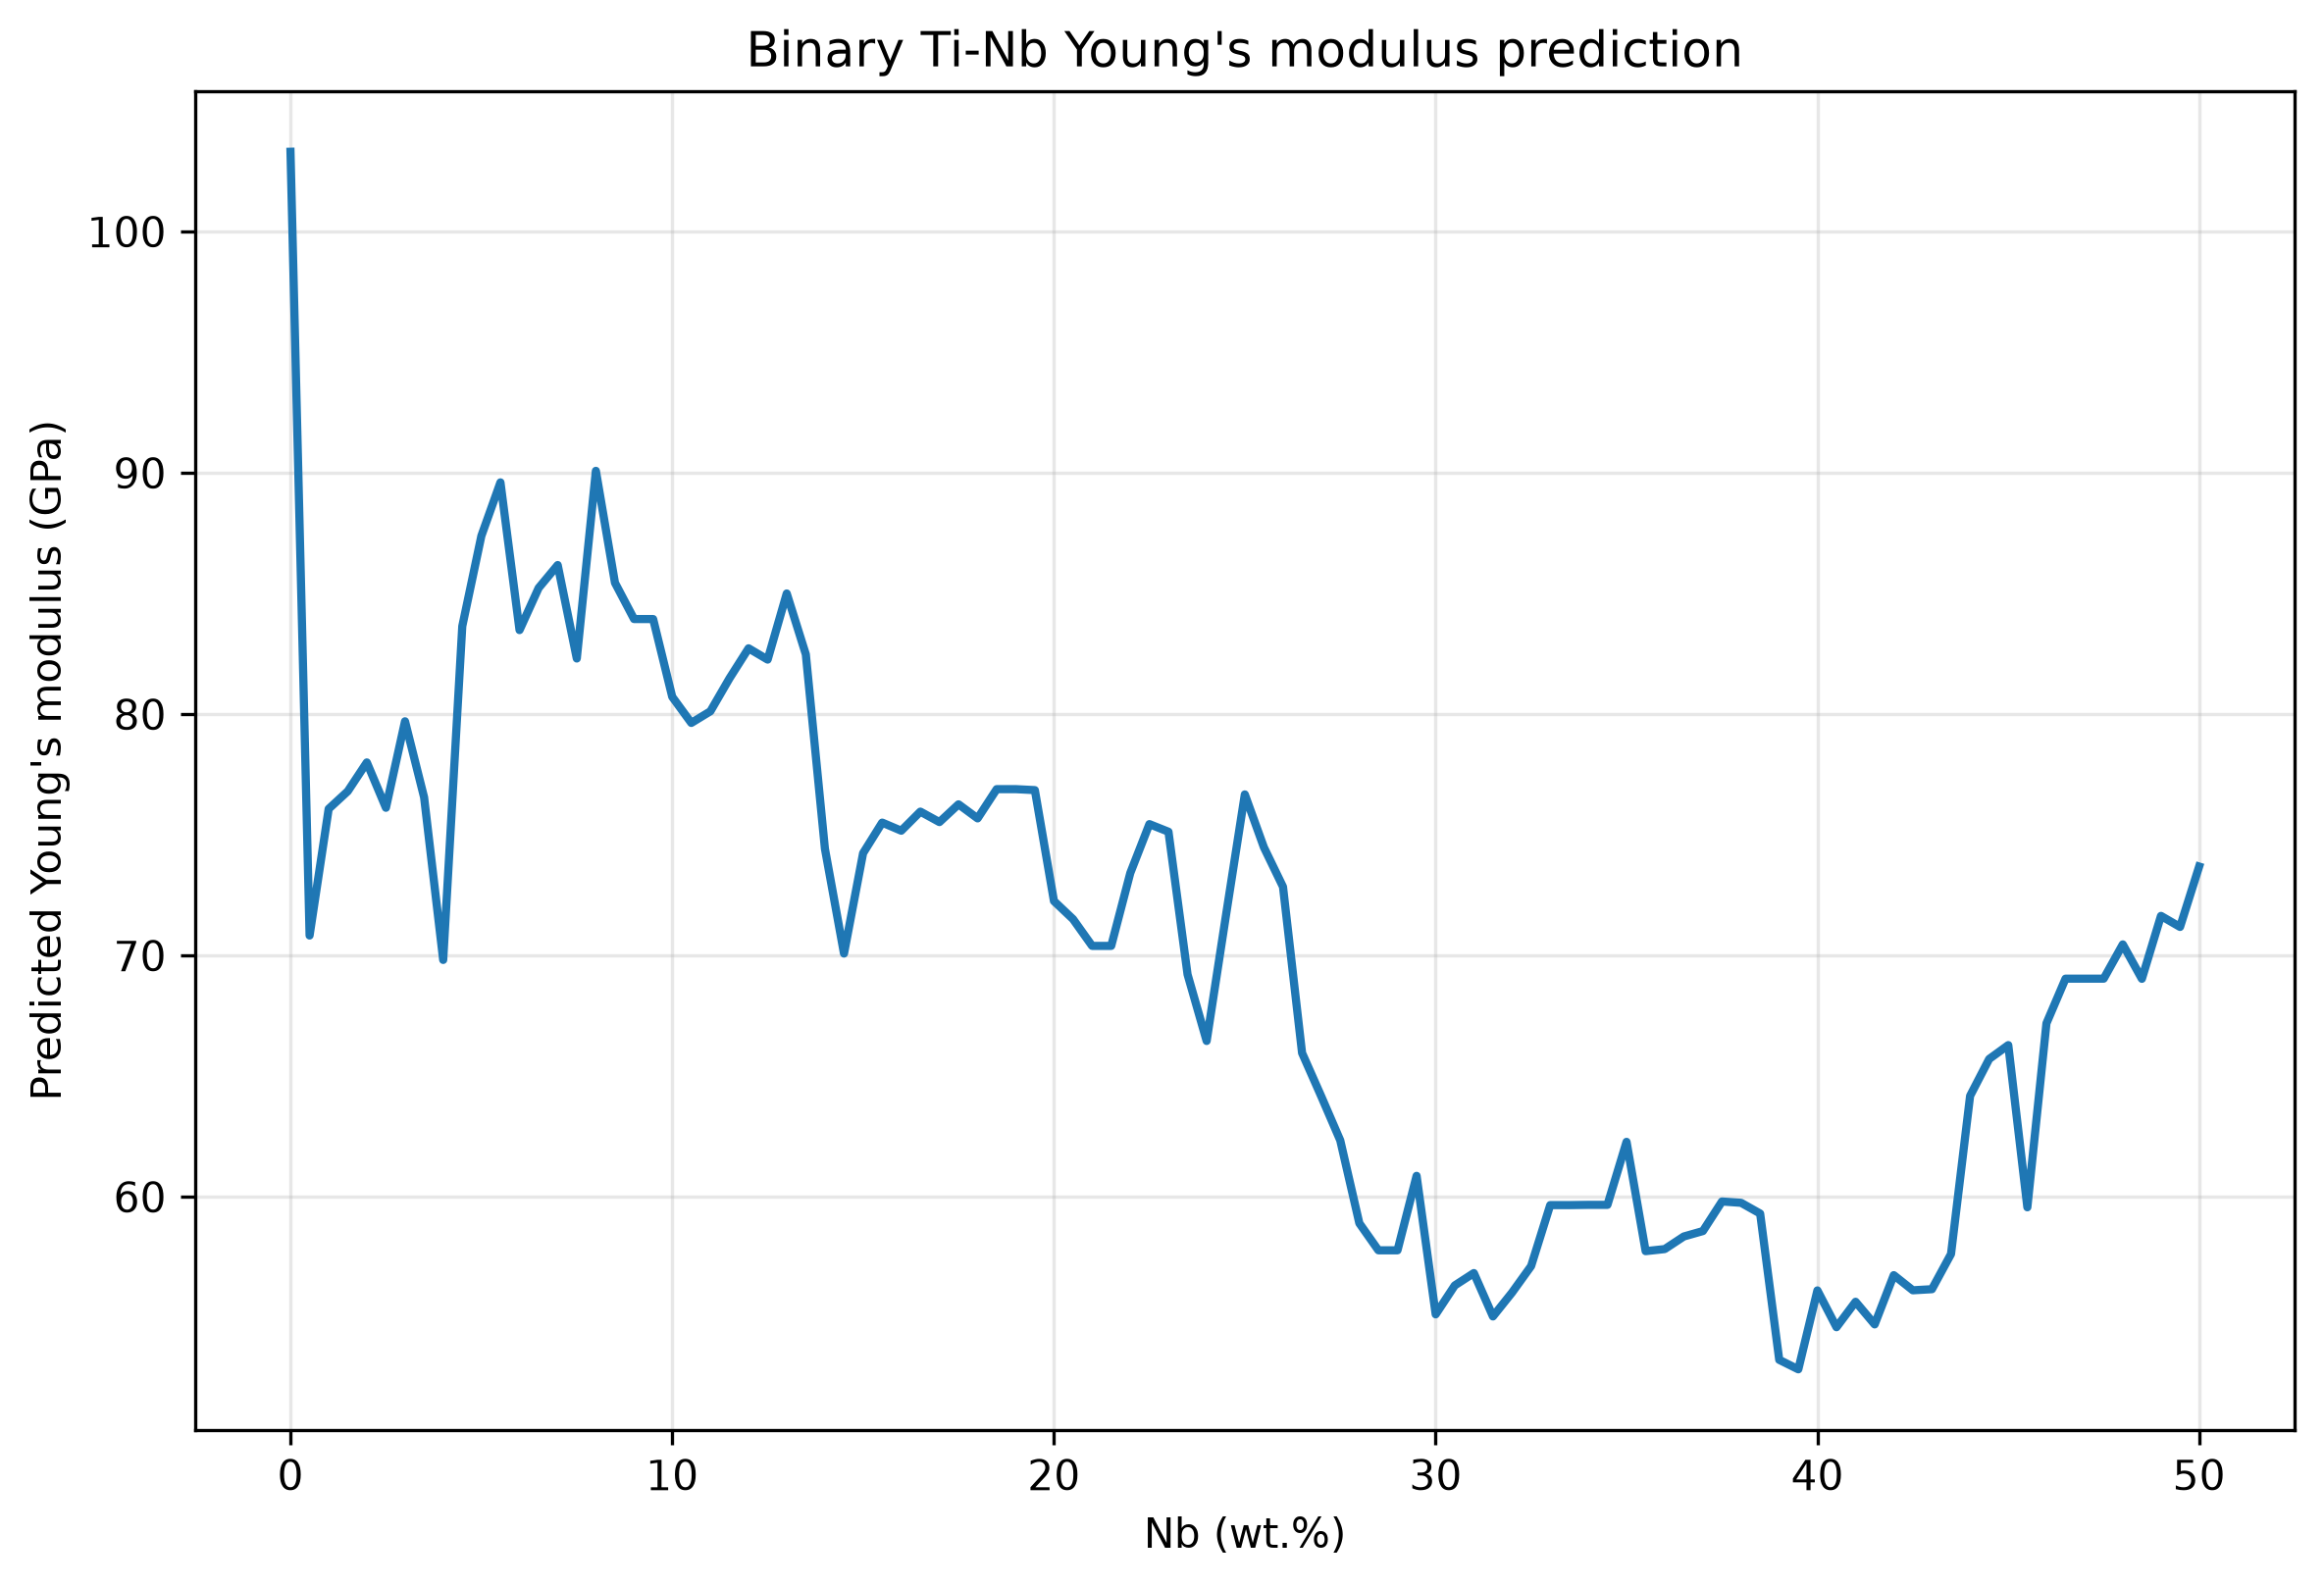
\includegraphics[width=0.82\linewidth]{nb_variation_graph.png}
\caption{Model-predicted Young's modulus across the binary Ti--Nb weight-composition sweep. The curve is model output, not a new experimental measurement.}
\label{fig:nb}
\end{figure}

\section{Discussion}
The test MAE of 9.88 GPa was about 1.12 times the estimated label-noise floor of 8.78 GPa. The gap indicates that the prediction error was of similar order to the within-composition variability observed in duplicate groups. The floor estimate was based on only 30 groups with repeated values and should not be interpreted as a universal measurement-noise limit.

The engineered features yielded a small average improvement over composition alone, but it was smaller than the fold-to-fold variability used for comparison. The model was therefore retained as a compact predictive baseline rather than evidence that the derived descriptors were intrinsically superior. The earlier model, before DFT exclusion, Ti-matrix filtering, and duplicate collapse, had a test MAE of 11.53 GPa and \(R^2=0.52\). Because the data preparation and split changed, this before/after comparison describes two pipeline runs and does not isolate a causal effect of any single cleaning step.

The largest errors were reported for dilute alloys with observed moduli around 91--113 GPa that the model predicted around 66--79 GPa. Examples included Ti--3Mo--1Nb, Ti--3Mo--1Al, Ti--7.4Cr, and Ti--8Mo--1Nb. Composition did not identify processing history or retained phase. As a result, alloys with similar chemistry but different conditions, such as quenched beta and annealed alpha+beta material, could have different moduli that the available features could not distinguish. [reference needed]

\section{Limitations}
The dataset combined measurements from tensile, ultrasonic, nanoindentation, and compression methods, together with values digitized from figures. Digitization carried estimated reading errors of approximately \(\pm 0.5\) to \(2\) GPa, while measurement protocols and processing histories were not harmonized. No processing, heat-treatment, or measured phase variable was included.

The phase label was a coarse screening feature derived from composition equivalents, not a measured phase state or thermodynamic calculation. XGBoost tree models produce stepwise responses and may not reproduce sharp phase-related modulus dips, including the reported 38.5 GPa value at Ti--14Nb--18Zr. The low-modulus test subset contained only 41 rows, so its MAE estimate was uncertain. Extrapolation beyond the training composition range was unreliable. Predictions should be treated as approximate, with an expected error of about \(\pm 10\) GPa, rather than as substitutes for measurements.

\section{Conclusion}
A grouped evaluation of composition-based models produced a test MAE of 9.88 GPa for the selected default XGBoost model using composition and engineered descriptors. The test \(R^2\) was 0.684. Engineered descriptors did not clearly outperform composition-only inputs by more than fold variability. The performance was close in scale to the empirical within-composition standard deviation, but incomplete process and phase information remained important limitations.

Future work should add processing and phase information, record source and measurement-method labels, obtain additional low-modulus beta-alloy experiments, and report calibrated uncertainty estimates. These additions would support a more discriminating evaluation of composition-based prediction.

\section*{References}
\noindent [reference needed: no bibliographic entries were supplied. Add the actual data-source papers and any standard references used before submission.]

\appendix
\section{Feature formulas and definitions}
Let \(x_i\) denote the atomic fraction of element \(i\), with \(\sum_i x_i=1\), and let \(r_i\) denote its metallic radius. Let \(r_{\mathrm{mean}}=\sum_i x_i r_i\). The composition was first normalized to 100 wt\% and then converted to atomic fractions using standard atomic masses. The definitions used were:
\begin{align}
\mathrm{VEC} &= \sum_i x_i\,\mathrm{VEC}_i,\\
\delta_r\;(\%) &= 100\sqrt{\sum_i x_i\left(1-\frac{r_i}{r_{\mathrm{mean}}}\right)^2},\\
\delta S_{\mathrm{mix}} &= -R\sum_i x_i\ln(x_i),\\
\mathrm{Mo}_{eq}\;(\mathrm{wt}\%) &= \mathrm{Mo}+0.2\mathrm{Ta}+0.28\mathrm{Nb}+0.4\mathrm{W}
+0.67\mathrm{V}+1.25\mathrm{Cr}+1.25\mathrm{Ni}+1.7\mathrm{Mn}
+1.7\mathrm{Co}+2.5\mathrm{Fe}-\mathrm{Al},\\
\mathrm{Al}_{eq}\;(\mathrm{wt}\%) &= \mathrm{Al}+\frac{\mathrm{Zr}}{6}
+\frac{\mathrm{Sn}}{3}+10\mathrm{O},\\
B_o &= \sum_i x_i B_{o,i},\qquad
M_d = \sum_i x_i M_{d,i}.
\end{align}
The ideal mixing entropy omitted terms for which \(x_i=0\). \(\mathrm{Mo}_{eq}\) and \(\mathrm{Al}_{eq}\) used weight-percent composition; VEC, \(\delta_r\), \(B_o\), and \(M_d\) used atomic fractions. The feature definitions and tabulated element constants require citations before external publication. [reference needed]

\begin{table}[H]
\centering
\caption{Model feature groups and phase-screening interpretation.}
\label{tab:features}
\begin{tabular}{p{0.20\linewidth}p{0.67\linewidth}}
\toprule
Feature group & Definition or interpretation\\
\midrule
Set A & Elemental composition columns in wt\%.\\
Set B & Set A plus VEC, \(\delta_r\), \(\delta S_{\mathrm{mix}}\), \(\mathrm{Mo}_{eq}\), \(\mathrm{Al}_{eq}\), \(B_o\), \(M_d\), and \texttt{phase\_est}.\\
\texttt{phase\_est} & \(\mathrm{Mo}_{eq}<2.5\) wt\%: alpha; \(2.5\) to \(10\) wt\% inclusive: alpha+beta; \(>10\) wt\%: beta. Marked uncertain when \(\mathrm{Al}_{eq}\geq 8\) wt\% or the alloy is Ti-poor (threshold not specified).\\
\bottomrule
\end{tabular}
\end{table}

\section{Numerical provenance}
All reported numerical values were supplied in the task description, except the 28/44 overlap count, which was calculated by comparing the supplied real-point list with \texttt{train\_v2.csv} using the requested tolerances. An accompanying audit file maps each reported value to its source statement in the task prompt. Author, affiliation, supervisor, date, and bibliography remain visible TODO items.

\end{document}
